\documentclass[aip, cp, amsmath, amssymb, reprint, nofootinbib]{revtex4-2}

\usepackage{graphicx}
\usepackage{dcolumn}
\usepackage{bm}

\usepackage{setspace}
\usepackage{graphicx}% Include figure files
\usepackage{fancyhdr}
\setlength{\parindent}{0in}

% Page Formatting
\pagenumbering{arabic} %\pagenumbering{gobble}
\onehalfspacing %doublespacing
\pagestyle{fancy}
%\usepackage{pdfpages}

% Heading Formatting
\headheight 32pt

% Link Formatting
\usepackage{hyperref}
\hypersetup{
	colorlinks,
	allcolors=black
	%citecolor=black,
	%filecolor=black,
	%linkcolor=black,
	%urlcolor=black
}


\usepackage{csvsimple}
\usepackage{mdframed}

\definecolor{commentsColor}{rgb}{0.497495, 0.497587, 0.497464}
\definecolor{keywordsColor}{rgb}{0.541176, 0.168627, 0.886275}
\definecolor{stringColor}{rgb}{0.000000, 0.558215, 0.135316}

% Code Formatting
\usepackage{listings}
\lstset
{ %Formatting for code
	basicstyle=\footnotesize\ttfamily,
	numbers=left,
	%caption={},
	%title={},
	stepnumber=1,
	showstringspaces=false,
	tabsize=1,
	breaklines=true,
	breakatwhitespace=false,
	frame=lines,
	xleftmargin=2em,
	framexleftmargin=1.5em,
	commentstyle=\color{commentsColor}\ttfamily,
  	stringstyle=\color{stringColor}\ttfamily,
	keywordstyle=\color{keywordsColor}\bfseries,
}
\newcommand{\lstprompt}{>\!>\!>}
\newcommand{\numberwithprompt}[1]{\footnotesize\ttfamily\selectfont \lstprompt}


% https://tex.stackexchange.com/questions/340232/how-insert-a-character-at-the-begin-of-every-line-from-a-source-code
\lstdefinestyle{console} {
	basicstyle=\footnotesize\ttfamily,
	numbers=left,
	stepnumber=1,
	showstringspaces=false,
	tabsize=1,
	breaklines=true,
	breakatwhitespace=false,
	frame=single,
	xleftmargin=2em,
	framexleftmargin=2.5em,
	%backgroundcolor=\color{gray!55},
	numberstyle=\numberwithprompt,
	}

% \lstdefinelanguage{psuedocode}{
%   keywords={typeof, new, true, false, catch, function, return, null, catch, switch, var, if, in, while, do, else, case, break},
%   keywordstyle=\color{blue}\bfseries,
%   ndkeywords={class, export, boolean, throw, implements, import, this},
%   ndkeywordstyle=\color{darkgray}\bfseries,
%   identifierstyle=\color{black},
%   sensitive=false,
%   comment=[l]{//},
%   morecomment=[s]{/*}{*/},
%   commentstyle=\color{purple}\ttfamily,
%   stringstyle=\color{red}\ttfamily,
%   morestring=[b]',
%   morestring=[b]"
% }

%\usepackage{algpseudocodex}
%Book Stuff

%\usepackage{algorithm}
%\usepackage[noend]{algpseudocode}
%\makeatletter
%\def\BState{\State\hskip-\ALG@thistlm}
%\makeatother

% Figures & Drawings
\usepackage{graphicx, caption}
\usepackage{animate}
\usepackage{tikz}
\usepackage{float}
\usepackage{pict2e}
\usepackage{subcaption}

% Physics
\usepackage{physics}

% Mathematics
\usepackage{amsmath}
\usepackage{amssymb}
\usepackage{amsthm}
\usepackage{mathtools}
%\usepackage{upgreek} % More Greek letters

% I don't really know what this is but I don't want to break shit
\usepackage{aliascnt}
\newaliascnt{eqfloat}{equation}
\newfloat{eqfloat}{h}{eqflts}
\floatname{eqfloat}{Equation}
\newcommand*{\ORGeqfloat}{}
\let\ORGeqfloat\eqfloat
\def\eqfloat{%
	\let\ORIGINALcaption\caption
	\def\caption{%
		\addtocounter{equation}{-1}%
		\ORIGINALcaption
	}%
	\ORGeqfloat
}
%}

% Bibliography (Citations) Formatting

%\usepackage{cite}
\usepackage{caption}
%\usepackage[backend=bibtex,style=verbose-trad2]{biblatex}
%works really really well, but no MLA format
%\usepackage[backend=biber]{biblatex}
%\bibliographystyle{apsrev4-1}
%\usepackage[backend=biber,style=mla]{biblatex} %Doesn't print all sources for some reason


%\usepackage{graphicx}% Include figure files
\usepackage{dcolumn}% Align table columns on decimal point
\usepackage{bm}% bold math
%\usepackage[mathlines]{lineno}% Enable numbering of text and display math
%\linenumbers\relax % Commence numbering lines

\usepackage[utf8]{inputenc}
\usepackage[T1]{fontenc}
%% Loads a Times-like font. You can also load
%% {newtxtext,newtxtmath}, but not {times}, 
%% {txfonts} nor {mathtpm} as these packages
%% are obsolete and have been known to cause problems.
\usepackage{mathptmx} 


\usepackage{amsthm}
\input{preamble/tikz}
\input{preamble/macros}


% ========================================= %
% LaTeX Template by Aditya K. Rao
% Contact at adi.rao@mail.utoronto.ca

% Change for each document [!!!]
\newcommand\course{PHY426}	% Course Code [!!!]
\newcommand\doctitle{Quantitative Verification of Thin Lense Equation} % Report Title [!!!]
\newcommand\firstauthorname{Report Author}
\newcommand\firstauthorstdnum{Student Number: 0000000000}
\newcommand\firstauthoremail{report.author@mail.utoronto.ca}
%\newcommand\secondauthorname{Author Two}
%\newcommand\secondauthorstdnum{Student Number: 0000000000}
%\newcommand\secondauthoremail{report.author@mail.utoronto.ca}
\newcommand\advname{Tahir Shaaran\space} % Advisor Name [!!!]  
\newcommand\taname{Sean Crawford\space} % Advisor Name [!!!] 

\newcommand{\location}{MP222} % Location [!!!]
% ========================================= %
 
% ============== EQUIPMENT ================ %

\newcommand{\oscope}{\texttt{DSOX1202G}\space}
\newcommand{\pdiode}{\texttt{DET36A2}\space}
\newcommand{\hene}{\texttt{HNLS008L}\space}
\newcommand{\cam}{\texttt{Alium 1800 U-500}\space}

% ========================================= %



%\pagenumbering{gobble}
\usepackage{listings}

\renewcommand\lstlistingname{Code Reference}
\renewcommand\lstlistlistingname{Code Reference}
\usepackage{tikz}
\usetikzlibrary{patterns}

\usepackage{circuitikz}

%\addbibresource{references.bib}
\usepackage{lipsum}
\usetikzlibrary{calc}

\begin{document}
\onecolumngrid
\pagenumbering{arabic}
\title{\doctitle}
\author{\firstauthorname}
\email{\firstauthoremail}
\thanks{\firstauthorstdnum}


%\email{report.author@mail.utoronto.ca}
%\thanks{Student Number: 0000000000}
\affiliation{
University of Toronto \\
\location, 60 St. George Street, Toronto, Ontario M5S 1A7, Canada.% Force line breaks with \\ if necessary
}

\date{\today} %Put in date of submission [!!!]

\preprint{APS/123-QED}
\begin{abstract}
    Multiple experiments were conducted to verify the focal lengths in various lenses.
\end{abstract}
    \maketitle
    %\tableofcontents 

    \lhead{\firstauthorname\vspace{0.1cm}}
    \chead{\textbf{\course} \\ \doctitle}
    \rhead{\textbf{Prof:} \advname \\ \textbf{TA:} \taname}
    \nocite{*}

    %\newpage
    \twocolumngrid
    \section{Introduction}
        % Plan
        % 1. Relavent Theory
        % 2. Simulation
        % 3. Talk about Hydrogen and Helium Emission Spectra, compare against lens data
        % 4. Talk about relavent theory for that
        % 5. Talk about the setup
        % Data Analysis and Relavent Results, make sure about unceratinties this time


        Optics and lesnes are a cornerstone of modern physics with their applications ranging from the study of the cosmos to the development of modern technology. However, the fundementals of such optical systems are often overlooked. In this experiment, the thin lens equation was quantiatively verified using a variety of lenses. The experiment was conducted in two parts. The first focused on verifying the thin lens equation, the second investigating if this still holds for thick lenses. Moreover, additional experimentation was conducted to investigate the diffraction patterns of light passing through a lens.

        \subsection{The Thin Lens Equation}

            The discovery of the thin lens equaton is of some debate. While the theory of lenses was well understood by the time of the ancient Greeks, some historians name Barrow (1669) and Huygens (1653) \cite{historyoptics} as accounting for some of the first semi-verbal descriptions of the thin lens equation. Such debate over \eqref{eqn:thinlens} is not suprising given its importance.

            \begin{equation} \label{eqn:thinlens}
                \frac{1}{f} = \frac{1}{p} + \frac{1}{q}
            \end{equation}

            \eqref{eqn:thinlens} describes the fundemental relationship between the focal length of a lens, the object distance, and the image distance. One may also derive the relationship with magnetization \eqref{eqn:mag}.

            \begin{equation} \label{eqn:mag}
                M = -\frac{q}{p}
            \end{equation}

            However, there is a fundemental assumption in both \eqref{eqn:thinlens} and \eqref{eqn:mag} which is that the lens is thin. In effect, this means that we approximate the lens as a 2D plane instead of a 3D object. In reality, a lens more acts as two seperate planes, a front plane and a back plane as can be seen in \figref{fig:real-lens}.

            \begin{figure}[H]
                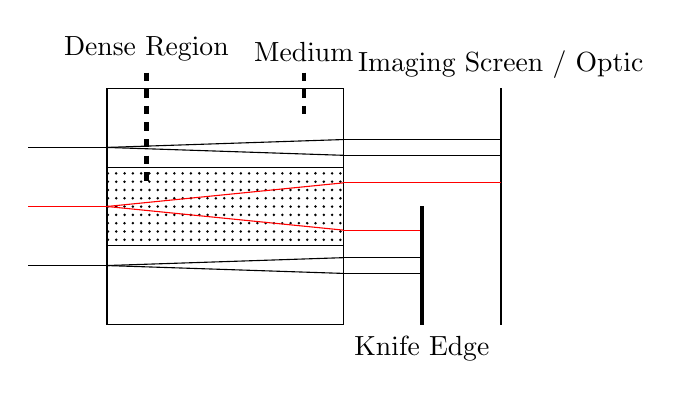
\begin{tikzpicture}
    \def\side{3}
    \def\height{3}
    \def\fmheight{2.5}
    \def\thick{0.25}
    \def\hpthick{0.5}

    \coordinate (TLC) at (-\side/2, \side/2);
    \coordinate (TRC) at (\side/2, \side/2);
    \coordinate (BLC) at (-\side/2, -\side/2);
    \coordinate (BRC) at (\side/2, -\side/2);

    \coordinate (TLC-dense) at ($(TLC)+(0,-1)$);
    \coordinate (TRC-dense) at ($(TRC)+(0,-1)$);
    \coordinate (BLC-dense) at ($(BLC)+(0,1)$);
    \coordinate (BRC-dense) at ($(BRC)+(0,1)$);

    % Draw Medium
    \draw (TLC) rectangle (BRC);

    % Dense Region
    \draw[pattern=dots] (TLC-dense) rectangle (BRC-dense);

    % Parallel Rays
    \draw ($(TLC)+(-1,-\side/4)$) -- ($(TLC)+(0,-\side/4)$);
    \draw[color=red] ($(TLC)+(-1,-\side/2)$) -- ($(TLC)+(0,-\side/2)$);
    \draw ($(TLC)+(-1,-3*\side/4)$) -- ($(TLC)+(0,-3*\side/4)$);

    % Refracting Rays
    \draw ($(TLC)+(0,-\side/4)$) -- ($(TRC)+(0,-\side/4+0.1)$);
    \draw[color=red] ($(TLC)+(0,-\side/2)$) -- ($(TRC)+(0,-\side/2+0.3)$);
    \draw ($(TLC)+(0,-3*\side/4)$) -- ($(TRC)+(0,-3*\side/4+0.1)$);

    % Refracting Rays
    \draw[color=black] ($(TLC)+(0,-\side/4)$) -- ($(TRC)+(0,-\side/4-0.1)$);
    \draw[color=red] ($(TLC)+(0,-\side/2)$) -- ($(TRC)+(0,-\side/2-0.3)$);
    \draw[color=black] ($(TLC)+(0,-3*\side/4)$) -- ($(TRC)+(0,-3*\side/4-0.1)$);

    % Refracted Rays
    \draw ($(TRC)+(0,-\side/4+0.1)$) -- ($(TRC)+(1,-\side/4+0.1)$);
    \draw[color=red] ($(TRC)+(0,-\side/2+0.3)$) -- ($(TRC)+(1,-\side/2+0.3)$);
    \draw ($(TRC)+(0,-3*\side/4+0.1)$) -- ($(TRC)+(1,-3*\side/4+0.1)$);
    
    % Refracted Rays
    \draw[color=black] ($(TRC)+(0,-\side/4-0.1)$) -- ($(TRC)+(1,-\side/4-0.1)$);
    \draw[color=red] ($(TRC)+(0,-\side/2-0.3)$) -- ($(TRC)+(1,-\side/2-0.3)$);
    \draw[color=black] ($(TRC)+(0,-3*\side/4-0.1)$) -- ($(TRC)+(1,-3*\side/4-0.1)$);

    % Knife Edge
    \coordinate (ket) at ($(TRC)+(1,0)$);
    \coordinate (kec) at ($(TRC)+(1,-\side/2)$);
    \coordinate (keb) at ($(BRC)+(1,0)$);

    \draw[ultra thick] (kec) -- (keb)node[anchor=north]{Knife Edge};

    
    % Screen
    \coordinate (scc) at ($(TRC)+(2,-\side/2)$);
    \coordinate (sct) at ($(TRC)+(2,0)$);
    \coordinate (scb) at ($(BRC)+(2,0)$);

    \draw[thick] (sct)node[anchor=south]{Imaging Screen / Optic} -- (scb);

    % Post Knife Edge Ray
    \draw ($(ket)+(0,-\side/4+0.1)$) -- ($(sct)+(0,-\side/4+0.1)$);
    \draw ($(ket)+(0,-\side/4-0.1)$) -- ($(sct)+(0,-\side/4-0.1)$);
    \draw[color=red] ($(ket)+(0,-\side/2+0.3)$) -- ($(sct)+(0,-\side/2+0.3)$);

    % Medium Label
    \draw[ultra thick, dashed] ($(TLC)+(2*\side/3+0.5,0.2)$)node[anchor=south]{Medium} -- ($(TLC)+(2*\side/3+0.5,-0.4)$);

    \draw[ultra thick, dashed] ($(TLC)+(\side/3-0.5,0.2)$)node[anchor=south]{Dense Region} -- ($(TLC)+(\side/3-0.5,-1.2)$);

\end{tikzpicture}
                \caption{Illustration of primary planes in a 3-dimension lens as inspired from the laboratory manual \cite{labmanual}.}
                \label{fig:real-lens}
            \end{figure}

        \subsection{The Thick Lens Equation}



        \subsection{Chromatic Abberations}



    \section{Methodology}

        The experiment was conducted using a 1.5 m optical bench equipped with a light source, diaphragms, lenses, and a screen. The apparatus was arranged in a classical object-lens-image configuration to investigate the thin lens equation. Three types of lenses—thin biconvex, spherical, and hemispherical—were studied.

        Proper alignment of the optical components was critical to ensure accurate measurements:

        \begin{enumerate}
            \item The lamp was positioned behind a diaphragm with a small aperture to produce a collimated beam.
            \item A screen was placed at a short distance from the diaphragm to check for alignment by marking the central light spot.
            \item The lens was positioned approximately 7 cm from the diaphragm, and its angle was adjusted to retro-reflect light back through the aperture.
            \item The screen was moved about 1 m away to observe the far-field focus, ensuring the beam remained centered.
            \item Fine adjustments were made iteratively to confirm proper alignment.
        \end{enumerate}


        The distances between optical elements were recorded using the built-in ruler of the optical bench. To account for systematic errors, offsets between the mount edges and the optical centers of the elements were measured using calipers with a precision of 0.1 mm. Uncertainties in these measurements were estimated by taking multiple readings and calculating the standard deviation.


        \subsection{Focal Length Estimation}
        The focal length of each lens was estimated through two methods:
        \begin{enumerate}
            \item Measuring the image distance when the lens was far from the light source.
            \item Using the lensmaker’s equation:
            \begin{equation}
                f = \frac{R}{2(n-1)}
            \end{equation}
            where $R$ is the radius of curvature and $n$ is the refractive index of the lens material.
        \end{enumerate}




\subsection{Data Collection}
A transparent grid was used as the object, and a screen was placed at varying distances to obtain a sharp focus. The following measurements were recorded:
\begin{itemize}
    \item Source, lens, and image positions along the optical bench.
    \item Image magnification by measuring the grid line spacing in the image.
    \item Multiple readings (3–5) for each configuration to determine uncertainty.
\end{itemize}
Data was collected for a range of object and image distances covering extreme cases ($q = f$ and $p = f$).

\subsection{Data Analysis and Iterative Improvements}
After an initial set of measurements, the data was plotted and analyzed to check consistency with the thin lens equation:
\begin{equation}
    \frac{1}{f} = \frac{1}{p} + \frac{1}{q}
\end{equation}

If inconsistencies were found, additional measurements were taken to refine the dataset. The analysis was conducted using MATLAB scripts (datacrunch.m and fitter.m), which performed least-squares fitting to determine the best estimates for lens parameters. The goodness-of-fit was evaluated using the chi-squared test.

\subsection{Thick Lens Measurements}
For thicker lenses, additional measurements were taken to determine whether the thin lens approximation remained valid. The locations of the front and back principal planes were estimated, and deviations from the ideal thin lens behavior were analyzed.


        \begin{figure}[H]
            \input{figures/expsetup-he.tex}
            \caption{Figure}
        \end{figure}


        \begin{figure}[H]
            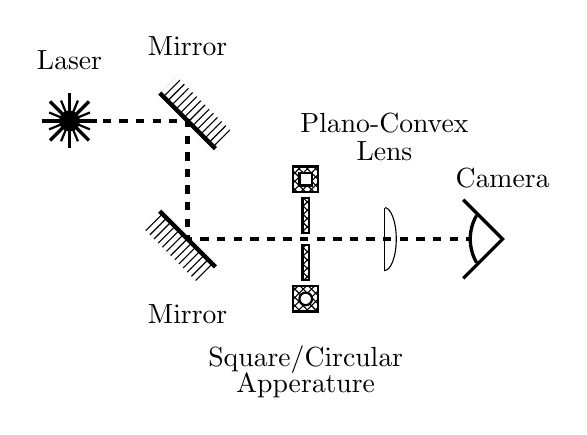
\begin{tikzpicture}
    \coordinate (L) at (0,0);
    \coordinate (M1) at (1.5,0);
    \coordinate (M2) at (1.5,-1.5);
    \coordinate (B) at (4,-1.5);
    \coordinate (A) at (3,-1.5);
    \coordinate (C) at (5.5,-1.5);

    % Laser Symbol
    \begin{scope}[scale=0.7]
        \draw[ultra thick, fill = black] (0,0) circle (0.15);
        \draw[rotate=0, very thick] (-0.5,0) -- (0.5,0);
        \draw[rotate=90, very thick] (-0.5,0) -- (0.5,0);
        \draw[rotate=45, very thick] (-0.5,0) -- (0.5,0);
        \draw[rotate=135, very thick] (-0.5,0) -- (0.5,0);

        \draw[rotate=22.5, thick] (-0.4,0) -- (0.4,0);
        \draw[rotate=67.5, thick] (-0.4,0) -- (0.4,0);
        \draw[rotate=112.5, thick] (-0.4,0) -- (0.4,0);
        \draw[rotate=157.5, thick] (-0.4,0) -- (0.4,0);
    \end{scope}


    % Mirror #1
    \begin{scope}[shift={(M1)}, rotate=-45]
        \draw[ultra thick] (-0.5,0) -- (0.5,0);
        \fill[pattern=north east lines] (-0.5,0) rectangle (0.5,0.30);
        %\coordinate (M1) at (0,-0.15);
    \end{scope}

    % Mirror #2
    \begin{scope}[shift={(M2)}, rotate=135]
        \draw[ultra thick] (-0.5,0) -- (0.5,0);
        \fill[pattern=north east lines] (-0.5,0) rectangle (0.5,0.30);
        %\coordinate (M2) at (0,-0.15);
    \end{scope}

    % Camera/Eye
    \begin{scope}[shift={(C)}, rotate=180]
        % Eye
        \draw[very thick] (0.5, 0.5) -- (0, 0) -- (0.5, -0.5);
        \draw[very thick] (0.33, -0.3) arc (-30:30:0.6);
    \end{scope}

    % Apperature
    \begin{scope}[shift={(A)}, scale=0.4]
        \draw[thick, pattern=crosshatch] (-0.1,1.3) rectangle (0.1,0.2);
        \draw[thick, pattern=crosshatch] (-0.1,-0.2) rectangle (0.1,-1.3);

        \draw[thick, pattern=crosshatch] (-0.4,1.5) rectangle (0.4, 2.3);
        \draw[thick, pattern=crosshatch] (-0.4,-1.5) rectangle (0.4, -2.3);

        \draw[thick, fill=white] (-0.2,1.7) rectangle (0.2, 2.1);
        \draw[thick, fill=white] (0,-1.9) circle (0.2);
    \end{scope}

    % Lens
    \begin{scope}[shift={(B)}, scale=0.5]
        %\draw[thick] (-0.3, -0.6) rectangle (0.3, 0.6);
        %\draw[dashed] (-0.5,-0.5) -- (0.5,0.5);
        %\coordinate (P1) at (0,0);
        \draw (0,0) ellipse (0.3 and 0.8);
        \filldraw[fill=white, color=white] (0,0.8) rectangle (-0.3,-0.8);
        \draw (0,0.8) -- (0,-0.8);
    \end{scope}

    % Laser Path
    \draw[ultra thick, dashed] (L) -- (M1) -- (M2) -- (A) -- (B) -- ($(C)-(0.4,0)$);

    % Labels
    \node[anchor=south, yshift=15] at (L) {Laser};
    
    \node[anchor=south, yshift=15] at (C) {Camera};
    
    \node[anchor=south, yshift=20] at (M1) {Mirror};
    
    \node[anchor=north, yshift=-20] at (M2) {Mirror};

    \node[anchor=north, yshift=-35] at (A) {Square/Circular};
    \node[anchor=north, yshift=-45] at (A) {Apperature};
    
    \node[anchor=south, yshift=35] at (B) {Plano-Convex};
    \node[anchor=south, yshift=25] at (B) {Lens};

\end{tikzpicture}
            \caption{Figure}
        \end{figure}



    \section{Results \& Analysis}
        
    
    \section{Discussion}
    
    
    \section{Conclusion}



    % Line to seperate report content from acknowledgements and references
\onecolumngrid
\begin{center}
    \vspace{0.8cm}
    \noindent\rule{0.9\textwidth}{0.5pt}
\end{center}

\begin{acknowledgments}
    The author would like to thank their supervisor, Prof. B. Braverman [11], for his guidance and support throughout the course of this experiment. Without his inisght much of the improvements as well as the suggenstion to measure free convection as opposed to the suggested setup would never have been possible. Additinonally, many thanks to Arya Kimiaghalam [12] (demonstrator) for developing ideas and providing futher suggestions as well as external processors to reach out to. The author would like to further acknowledge the support of the lab technician team L. Avramidis and P. Scolieri. Finally, the support of author experimentors in MP247 should be acknowledged as they provided valuable feedback and suggestions for the experiment.
\end{acknowledgments}

\bibliography{references}

\appendix
\section{Appendix}
\subsection{Raw Data}

\subsection{Analysis Code}

\end{document}